\section{La technique}
\subsection{Configuration minimale}
\begin{frame}
  \frametitle{\color{white} Configuration minimale}
  \begin{block}{Matériel}
    \begin{itemize}
      \item Processeur 1GHz.
      \item 512 Mo de RAM.
      \item 3 Mo d'espace disque.
    \end{itemize}
  \end{block}
  \begin{block}{Système d'exploitation}
    \begin{itemize}
      \item GNU Linux avec environnement graphique.
      \item Windows.
    \end{itemize}
  \end{block}
  \begin{block}{Logiciels}
    \begin{itemize}
      \item GNU Privacy Guard (GPG) version 1.4 ou supérieure.
      \item Qt 5.
    \end{itemize}
  \end{block}
\end{frame}

\subsection{Outils de développement}
\begin{frame}
  \frametitle{\color{white} Outils de développement}
  \begin{block}{Langage}
    \begin{itemize}
      \item C++ 11.
      \item Qt 5.
    \end{itemize}
  \end{block}
  \begin{block}{Pourquoi le C++ 11 ?}
    \begin{itemize}
      \item Rapidité d'exécution.
      \item Communication simplifiée avec GPG.
      \item Langage natif de Qt.
    \end{itemize}
  \end{block}
  \begin{block}{Pourquoi Qt 5 ?}
    \begin{itemize}
      \item Cadriciel multiplate-forme.
      \item KDE est basé sur ce cadriciel.
    \end{itemize}
  \end{block}
\end{frame}
\subsection{Architecture}
\begin{frame}
  \frametitle{\color{white} Architecture}
  \begin{block}{Patron de conception}
    \begin{itemize}
      \item Modèle - Vue.
      \item Utilisé par Qt pour ses composants d'interface graphique.
    \end{itemize}
  \end{block}
  \begin{figure}[p]
    \centering
    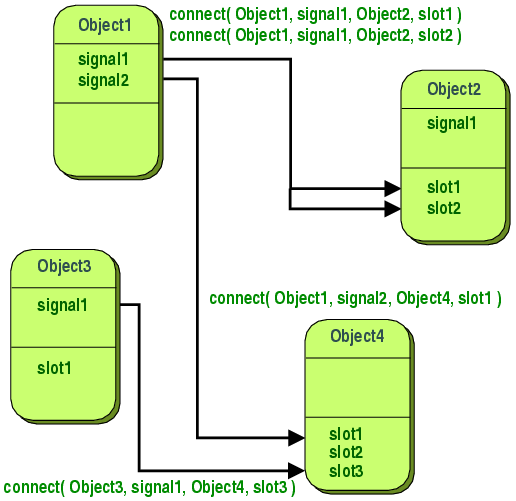
\includegraphics[scale=.25]{MV.png}
    \caption{Signaux et Slots Qt}
  \end{figure}
\end{frame}
